\section{Сравнение моделей}

\subsection{Показатели качества}

Для трёх построенных моделей вычислены следующие показатели качества.

Коэффициент детерминации:

\[
R^2 = 1 - \frac{RSS}{TSS},
\]
где
\[
TSS = \sum_{i=1}^{n}(y_i - \bar{y})^2 = 34\,322\,573.926, \quad
RSS = \sum_{i=1}^{n}(y_i - \hat{y}_i)^2.
\]

Средняя ошибка аппроксимации:

\[
A = \frac{100\%}{n}\sum_{i=1}^{n}\left|\frac{y_i - \hat{y}_i}{y_i}\right|.
\]

\subsection{Сводная таблица}

В таблице~\ref{tab:comparison} представлены значения показателей для всех трёх моделей.

\begin{table}[H]
\centering
\caption{Сравнение моделей по качеству аппроксимации}
\label{tab:comparison}
\begin{tabular}{lcc}
\toprule
Модель & \(R^2\) & \(A\), \% \\
\midrule
Линейная \(y = a + bx\) & 0.7446 & 18.85 \\
Квадратичная \(y = a + bx + cx^2\) & 0.7542 & 18.36 \\
Степенная \(y = ax^b\) & 0.7401 & 16.74 \\
\bottomrule
\end{tabular}
\end{table}

\subsection{Анализ остатков}

На рисунке~\ref{fig:residuals} представлены графики остатков для трёх моделей.

\begin{figure}[H]
\centering
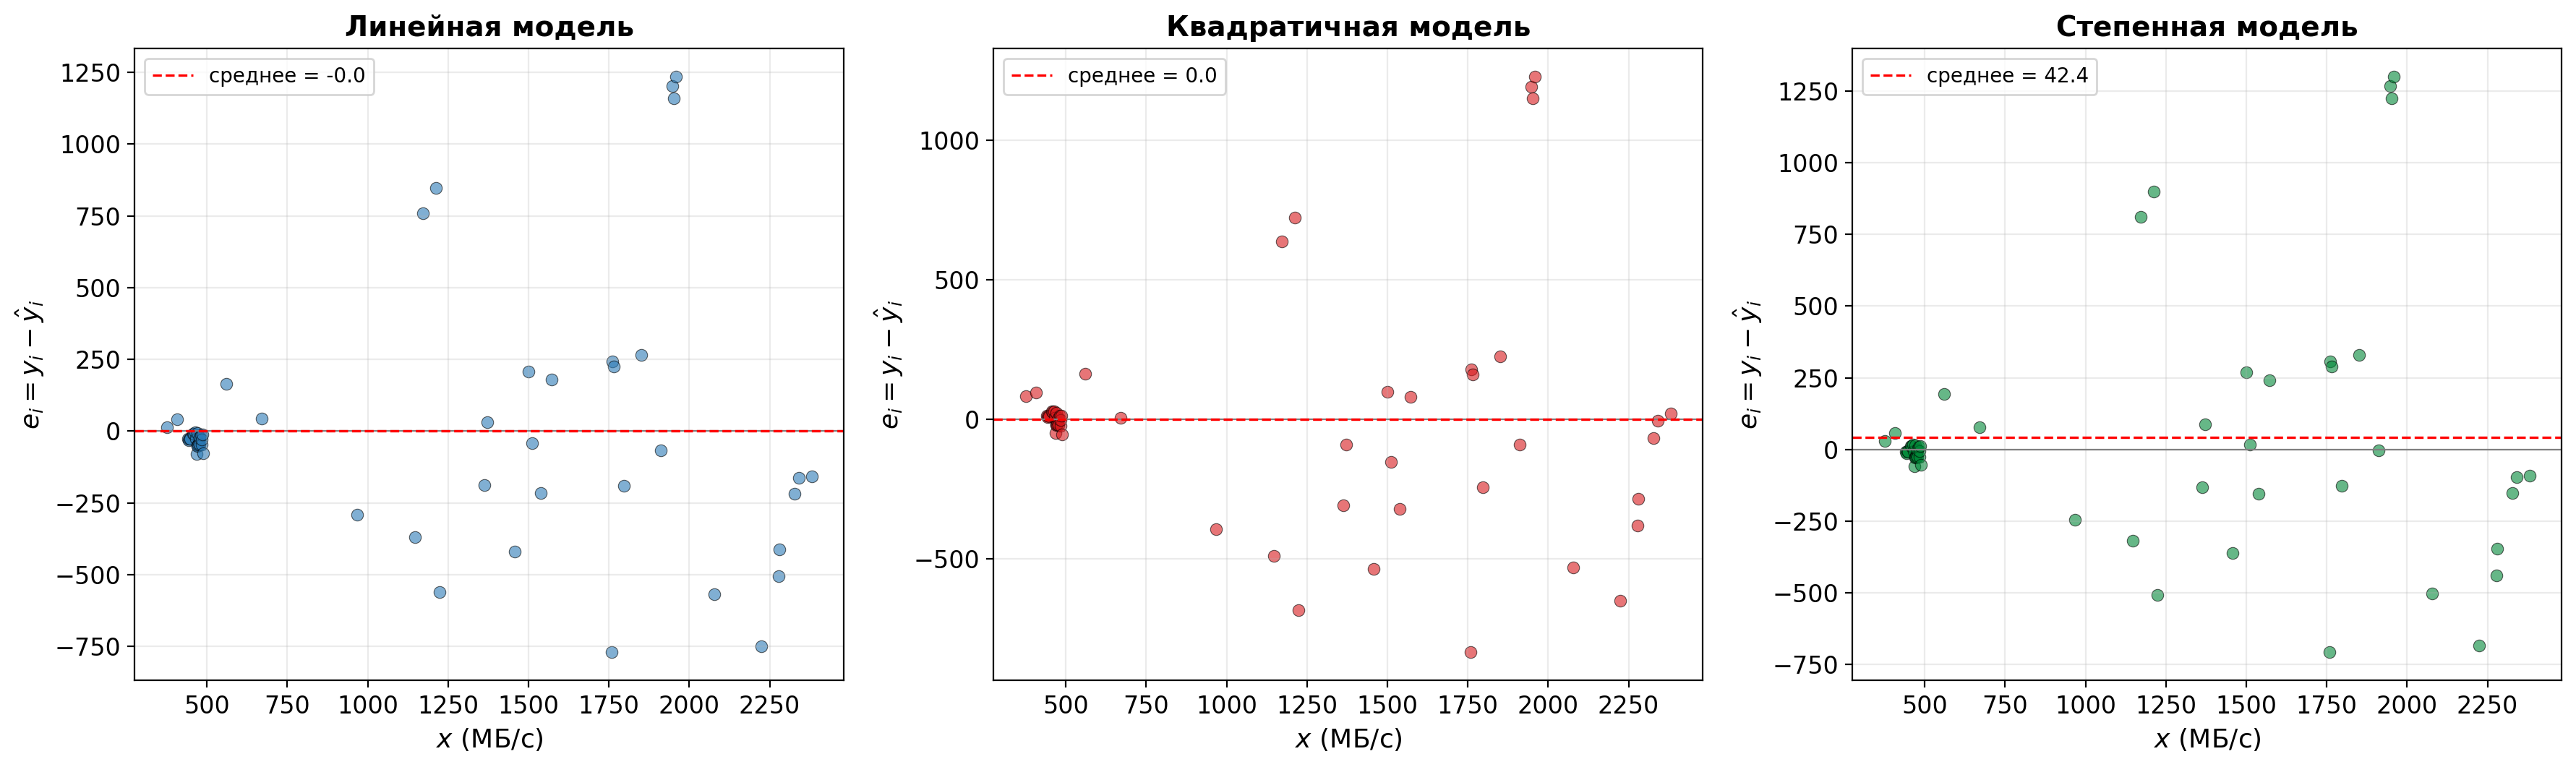
\includegraphics[width=0.95\textwidth]{residuals.png}
\caption{Графики остатков \(e_i = y_i - \hat{y}_i\) для трёх моделей}
\label{fig:residuals}
\end{figure}

Анализ графиков остатков и численных характеристик (\(e_i = y_i - \hat{y}_i\)) показывает:

\begin{itemize}
    \item \textbf{Линейная модель:} остатки демонстрируют выраженный систематический паттерн. При малых \(x\) (\(x < 500\)) остатки преимущественно \textbf{отрицательны} (среднее \(\approx -27.7\)); в средней области (\(500 < x < 1500\)) — также преобладают отрицательные значения; при \(x \approx 1950\) наблюдается компактная группа из трёх точек с экстремально большими положительными остатками (\(>1100\)), соответствующих аномально высоким значениям \(y\) (более 3000 МБ/с); при \(x > 2000\) остатки вновь становятся отрицательными. Баланс знаков: 15 положительных против 39 отрицательных — ярко выраженный перекос в отрицательную сторону.

    \item \textbf{Квадратичная модель:} по сравнению с линейной, квадратичная модель существенно улучшает баланс остатков: 28 положительных и 26 отрицательных (близко к равномерному распределению знаков). Средний остаток в нижней половине значений \(x\) составляет \(-1.93\) против \(-27.74\) у линейной модели. Добавление квадратичного члена частично компенсирует систематическое занижение в области малых \(x\), однако при этом модель по-прежнему плохо описывает три выброса при \(x \approx 1950\) и даёт значительные отрицательные остатки при \(x > 2000\).

    \item \textbf{Степенная модель:} в области малых \(x\) (\(x < 500\)) средний остаток близок к нулю (\(-0.75\)), что говорит о хорошем согласии модели с данными в этой зоне. Характер остатков наиболее близок к случайному (25 смен знака — наибольшее среди трёх моделей), однако имеется систематическое положительное смещение на всём диапазоне (\(\sum e_i \approx 2290\), среднее \(\approx 42.4\)), связанное с тем, что модель оценивалась на логарифмической шкале и не гарантирует несмещённости после обратного преобразования. При больших \(x\) разброс остатков также увеличивается (гетероскедастичность), хотя и не столь резко, как у линейной модели в окрестности выбросов.
\end{itemize}

\subsection{Сравнительный график}

На рисунке~\ref{fig:comparison} все три модели наложены на исходные данные.

\begin{figure}[H]
\centering
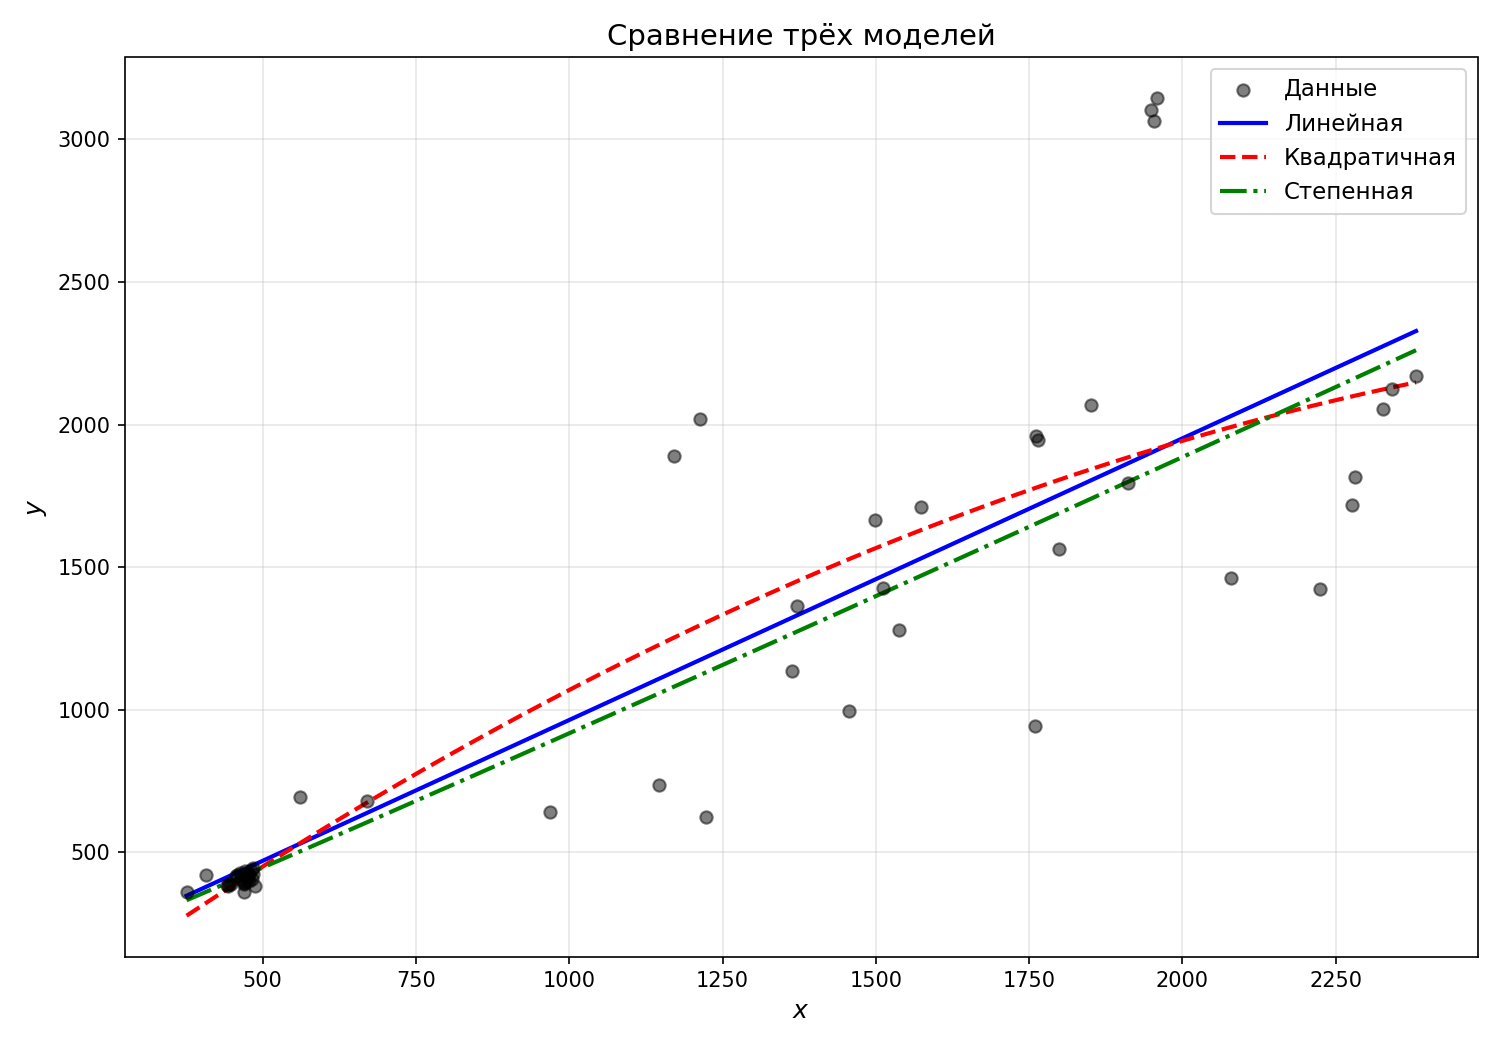
\includegraphics[width=0.85\textwidth]{comparison.png}
\caption{Сравнение трёх регрессионных моделей}
\label{fig:comparison}
\end{figure}

\subsection{Выбор лучшей модели}

По совокупности критериев:
\begin{itemize}
    \item по коэффициенту детерминации \(R^2\) наилучшей является \textbf{квадратичная} модель (\(R^2 = 0.7542\));
    \item по средней ошибке аппроксимации \(A\) наилучшей является \textbf{степенная} модель (\(A = 16.74\%\));
    \item линейная модель уступает двум другим по обоим показателям, однако различие невелико (\(R^2 = 0.7446\) против 0.7542 у лучшей).
\end{itemize}

С учётом всех критериев \textbf{степенная модель \(y = ax^b\) представляется наиболее предпочтительной}: она имеет наименьшую среднюю ошибку аппроксимации (\(A = 16.74\%\)), наилучшее согласие с данными в области малых \(x\) (средний остаток \(-0.75\)), а её остатки демонстрируют наиболее случайный характер (25 смен знака). Квадратичная модель, несмотря на чуть более высокий \(R^2\) и лучший баланс знаков остатков (28/26), содержит отрицательный квадратичный член, который приводит к убыванию прогноза при больших \(x\), что противоречит физическому смыслу зависимости скорости записи от скорости чтения SSD. Линейная модель наиболее проста, однако её остатки имеют явно выраженный систематический характер.

Линейная модель при этом остаётся полезной как наиболее простая и хорошо изученная; для неё далее будет выполнен подробный статистический анализ.
